\chapter{Planificación}\label{sec:plani}

\lettrine{A} continuación se detallan las fases seguidas en el proyecto, subdividiendo la gestión en las dos ramas principales del mismo: análisis de sentimientos y servicio web.

\section{Análisis de sentimientos}

\subsection{Fase 1: Inicio}

Se trata de una fase de documentación y aprendizaje.

En esta fase se realizará un análisis del estado del arte del problema, además se estudiará cuales son las tecnologías más comunes para abordarlo, y se tratará de familiarizarse con el dominio de la tarea.

\subsection{Fase 2: Elaboración}

Se establecen una serie de requisitos a cumplir por el clasificador, y se establecen los casos de uso. Posteriormente se realiza un primer modelado de la estructura de clases, que será posible que cambie según se vayan presentando nuevas posibilidades de experimentos a realizar.

\subsection{Fase 3: Construcción}

Se comienza la implementación del código, esta fase constará de varias iteraciones que irán sumando funcionalidades al sistema.

\paragraph{Iteración 1} En esta iteración se comenzará por la implementación de un algoritmo de clasificación que sirva como línea base. Además será necesario implementar el algoritmo de tratamiento del corpus de documentos, será necesario pasar de formato XML a un formato que sea válido como entrada de los clasificadores, en este caso se ha elegido un tipo DataFrame de Python, que nos facilitará el tratamiento posterior de los textos.

\paragraph{Iteración 2} Se procederá a implementar la clase de preprocesamiento de los textos que nos servirá para probar métodos para aumentar la eficacia del clasificador.

\paragraph{Iteración 3} Se desarrollarán una serie de estudios sobre los datos y las posibilidades de mejora tanto del preprocesado como de los algoritmos, partiendo de los resultados de la línea base.

\paragraph{Iteración 4} Se creará una clase capaz de procesar los resultados, y ofrecer recursos visuales de valor que nos ayuden a comparar los resultados obtenidos. 

\subsection{Fase 4: Fase de transición}
Con el programa listo se procederá a realizar las ejecuciones de los modelos y obtener unos datos que servirán para hacer una comparativa de los mismos. Como consecuencia de estos resultados se decidirá si es necesario corregir errores, buscar nuevos modelos o consideramos que el programa está ya listo para su entrega.

Es posible que tras finalizar esta fase veamos necesario volver a la fase anterior, ya sea por necesidad de corregir errores, o porque durante la investigación se ha descubierto alguna otra estrategia que se estime pueda funcionar mejor que la adoptada hasta ahora.

\section{Servicio web}

\subsection{Fase 1: Fase de inicio}
Dado que abordaremos la implementación de una sección de una página Web perteneciente a un proyecto ya existente, en esta primera fase trataremos de comprender el funcionamiento y la estructuración del código ya existente, posteriormente se hará un análisis de los requisitos del módulo.

\subsection{Fase 2: Fase de elaboración}

Tras haber comprendido el sistema existente y haber refinado los requisitos, procederemos a la extracción de los casos de uso, del modelo de base de datos y del modelado de clases.

\subsection{Fase 3: Fase de construcción}

Con toda la documentación establecida se procederá a la implementación de las funcionalidades del módulo siguiendo un ciclo de iteraciones.

\paragraph{Iteración 1} Se implementará en el servidor las operaciones CRUD\footnote{CRUD: Create Read Update Delete} de la entidad Comentario, así como los endpoints que permitirán al cliente acceder a estos servicios.

\paragraph{Iteración 2} Se creará la vista principal del módulo de comentarios que permitirá al usuario acceder a una lista de los mismos desde el perfil de cada producto.

\subsection{Fase de transición}

Se realizarán las pruebas finales para verificar que el módulo funciona tal y como se establece en los requisitos y que todos los casos de uso están implementados de forma correcta.

\section{Diagrama de Gantt}

\begin{figure}[!ht]
	\centering
	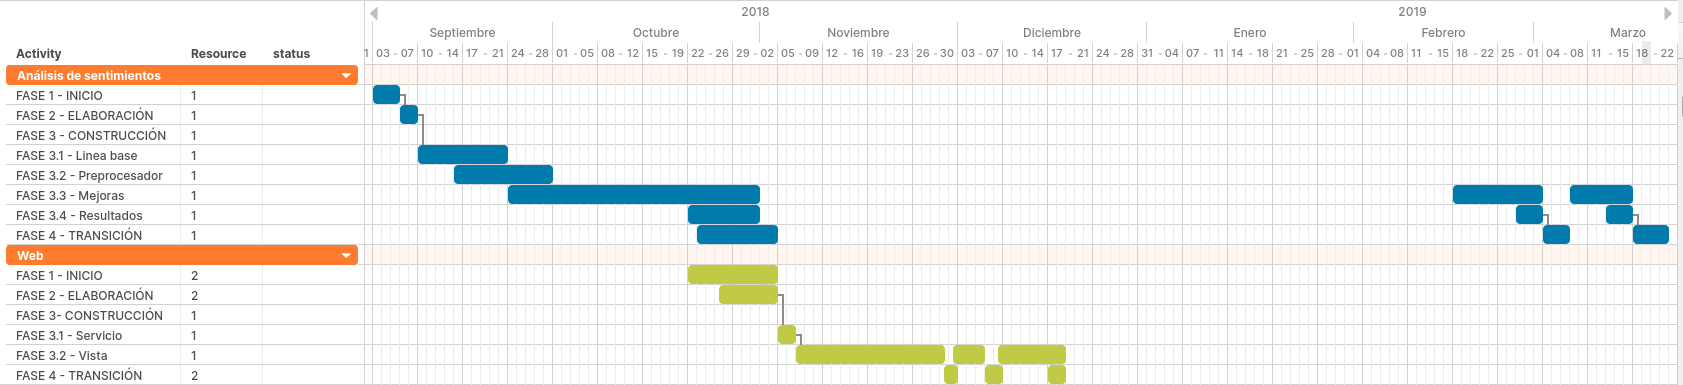
\includegraphics[width=0.75\textwidth]{imaxes/gantt.png}
	\caption{Diagrama de Gantt del proyecto (BCS).}
	\label{gant}
\end{figure}

El diagrama de Gantt realizado para el proyecto (fig. \ref{gant}) representa los tiempos de desarrollo en un BCS (Best Case Scenario).

En esta casuística el proyecto podría durar hasta 4 meses de desarrollo como mínimo, aunque en el diagrama se incluye la posibilidad de encontrar algún fallo o método de clasificación más eficaz meses más tarde.

Como vemos las tareas no tienen por qué ser secuenciales, dado que si suponemos que la carga prevista de la tarea va a ser baja podemos paralelizarla con otra, y en muchos casos la propia naturaleza de la tarea nos obligará a ejecutarla de forma paralela, ya que, por ejemplo la construcción del preprocesador de textos se verá influida por los resultados obtenidos en la clasificación y viceversa.

En cuanto a la parte final del desarrollo web vemos que se intercalan la fase 4 y la fase 3.2, esto se debe a que esperamos encontrar fallos en las fases de prueba que necesitarán ser corregidos y probados de nuevo.

En el desarrollo real de este proyecto se ha entregado el PVM (Producto Viable Mínimo) dentro del tiempo especificado en la estimación. Sin embargo se han realizado varios ciclos de desarrollo posteriores para mejorar la implementación de ciertos algoritmos, mediante prueba de nuevas tecnologías, corrección de errores o afinación de hiperparámetros. Estos esfuerzos sumarán un total de 192 horas imputables a las tareas 3.3 y 3.4 del análisis de sentimientos.

\section{Estimación de recursos}

Para la realización de este proyecto se necesitarán al menos 2 personas con 2 roles diferenciados, un analista que se encargue de la recogida de requisitos y diseño inicial del sistema y un programador que lo implemente.

En caso de ser necesario podríamos recurrir a un tercer recurso para la realización de la investigación, que bien podría ser un ingeniero de datos o un especialista en el campo del aprendizaje automático.

\section{Estimación de costes}

Para realizar la estimación de costes vamos a tener en cuenta la participación de dos recursos, un analista en las fases iniciales del desarrollo web y un programador junior a lo largo de todo el proyecto. Los cálculos se realizarán sobre la estimación inicial, sin tener en cuenta el tiempo de desarrollo fuera del escenario BCS.

Los recursos tendrían una remuneración de:

\begin{itemize}
	\item Analista: 17€/hora
	\item Programador: 12€/hora
\end{itemize}

A continuación se muestran las tablas con la estimación de esfuerzo de los recursos durante los tres meses y medio estimados como mejor escenario posible, separadas por subsitemas.

\begin{table}[H]
	\centering
\begin{tabular}{|l|c|c|c|}
	\hline
	Tarea  & Precio (€/hora) & Esfuerzo aprox. (horas) & Total (€) \\ \hline
	FASE 1 & 12              & 24                      & 288       \\ \hline
	FASE 2 & 12              & 16                      & 192       \\ \hline
	FASE 3 & 12              & 384                      & 3072       \\ \hline
	&                 & 424 h                    & 3552 €    \\ \hline
\end{tabular}
\caption{Estimación de esfuerzo subsistema de análisis de sentimientos.}
\label{esf-anal-sent}
\end{table}

\begin{table}[H]
	\centering
	\begin{tabular}{|l|c|c|c|}
		\hline
		Tarea  & Precio (€/hora) & Esfuerzo aprox. (horas) & Total (€) \\ \hline
		FASE 1 & 17              & 80                      & 1360      \\ \hline
		FASE 2 & --              & 56                      & --        \\ \hline
		FASE 3 & 12              & 256                     & 3072      \\ \hline
		&                 & 336 h                   & 4432 €    \\ \hline
	\end{tabular}
\caption{Estimación de esfuerzo desarrollo aplicación web.}
\label{esf-web}
\end{table}

Como vemos en la tabla \ref{esf-web} en las primeras fases solo se ha tenido en cuenta el trabajo realizado por el analista, ya que el programador tendrá que paralelizar esta etapa con la fase final del otro subsistema. Además dado que el analista paralelizará su trabajo en estas primeras fases la fase 2 de 56 horas no supondrá un costo a mayores.

Teniendo estos datos en cuenta podemos estimar un coste de 7.984 € para el proyecto. Si además sumamos el costo de las 192 horas asignadas al programador para un posible caso de arreglo o mejora futura obtenemos un total de 10.288€.




